%% mtalk-example.tex -- example for the mtalk class (beamer + Moloch).
%%
%% Build with latexmk (two runs are needed, see doc/NOTES.md).
%% Class options: "dark" for the dark Moloch background, "nocharter" to keep
%% Moloch's own sans body font instead of Bitstream Charter.
\documentclass{mtalk}

\usepackage{mstuff}

\title{Ableitungen}
\subtitle{Eine Einführung}
\author{Marc Schlienger}
\institute{Rolf-Benz-Schule Nagold}
\date{\today}

\license{\href{https://creativecommons.org/licenses/by/4.0}{CC BY 4.0}}
%\mtalksetup{logo=Rolf-Benz-Schule.png}

%%%%%%%%%%%%%%%%%%%%%%%%%%%%%%%%%%%%%%%%%%%%%%%%%%%%%%%%%%%%%%%%%%%%%%%%%%%%%%
\begin{document}

\maketitle

\section{Grundlagen}

\begin{frame}{Der Differenzenquotient}
	\begin{itemize}
		\item Die Sekantensteigung durch zwei Punkte
		\item Der Grenzübergang $h \to 0$
	\end{itemize}
	\[ f'(x_0) = \lim_{h \to 0}\frac{f(x_0+h)-f(x_0)}{h} \]
\end{frame}

\begin{frame}{Merksatz und Beispiel}
	\begin{mrule}[Merksatz]
		Die Ableitung an der Stelle $x_0$ ist die Steigung der Tangente.
	\end{mrule}
	\begin{mexample}[Beispiel]
		Für $f(x)=x^2$ ist $f'(x)=2x$.
	\end{mexample}
\end{frame}

\section{Anwendung}

\begin{frame}{Ein Schaubild}
	\centering
	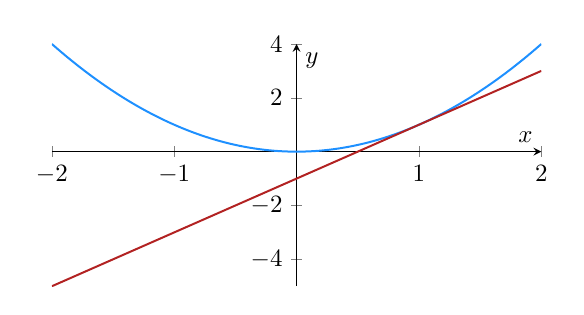
\begin{tikzpicture}[scale=0.9]
		\begin{axis}[axis lines=middle, xlabel=$x$, ylabel=$y$,
			width=0.7\linewidth, height=5cm, domain=-2:2, samples=100]
			\addplot[thick, DodgerBlue] {x^2};
			\addplot[thick, FireBrick] {2*x-1};
		\end{axis}
	\end{tikzpicture}
\end{frame}

\begin{frame}{Zwei Spalten}
	\begin{columns}[T]
		\begin{column}{0.48\linewidth}
			\textbf{Ableitung}
			\begin{itemize}
				\item Steigung der Tangente
				\item lokale Änderungsrate
			\end{itemize}
		\end{column}
		\begin{column}{0.48\linewidth}
			\textbf{Integral}
			\begin{itemize}
				\item Fläche unter dem Graphen
				\item Rekonstruktion des Bestands
			\end{itemize}
		\end{column}
	\end{columns}

	\bigskip
	Wichtig ist der \alert{Grenzübergang}.
\end{frame}

\begin{frame}{Beamer-Blöcke}
	\begin{block}{Satz}
		Ist $f$ differenzierbar, so ist $f$ stetig.
	\end{block}
	\begin{alertblock}{Achtung}
		Die Umkehrung gilt nicht.
	\end{alertblock}
	\begin{exampleblock}{Gegenbeispiel}
		$f(x) = |x|$ ist stetig, aber nicht differenzierbar in $0$.
	\end{exampleblock}
\end{frame}

\begin{frame}[standout]
	Fragen?
\end{frame}

\end{document}
